\section{BFM-Zero for Humanoid Whole-body Control}\label{sec:training}
\vspace{-2mm}
\begin{figure}[htbp]
    \begin{center}
    \centerline{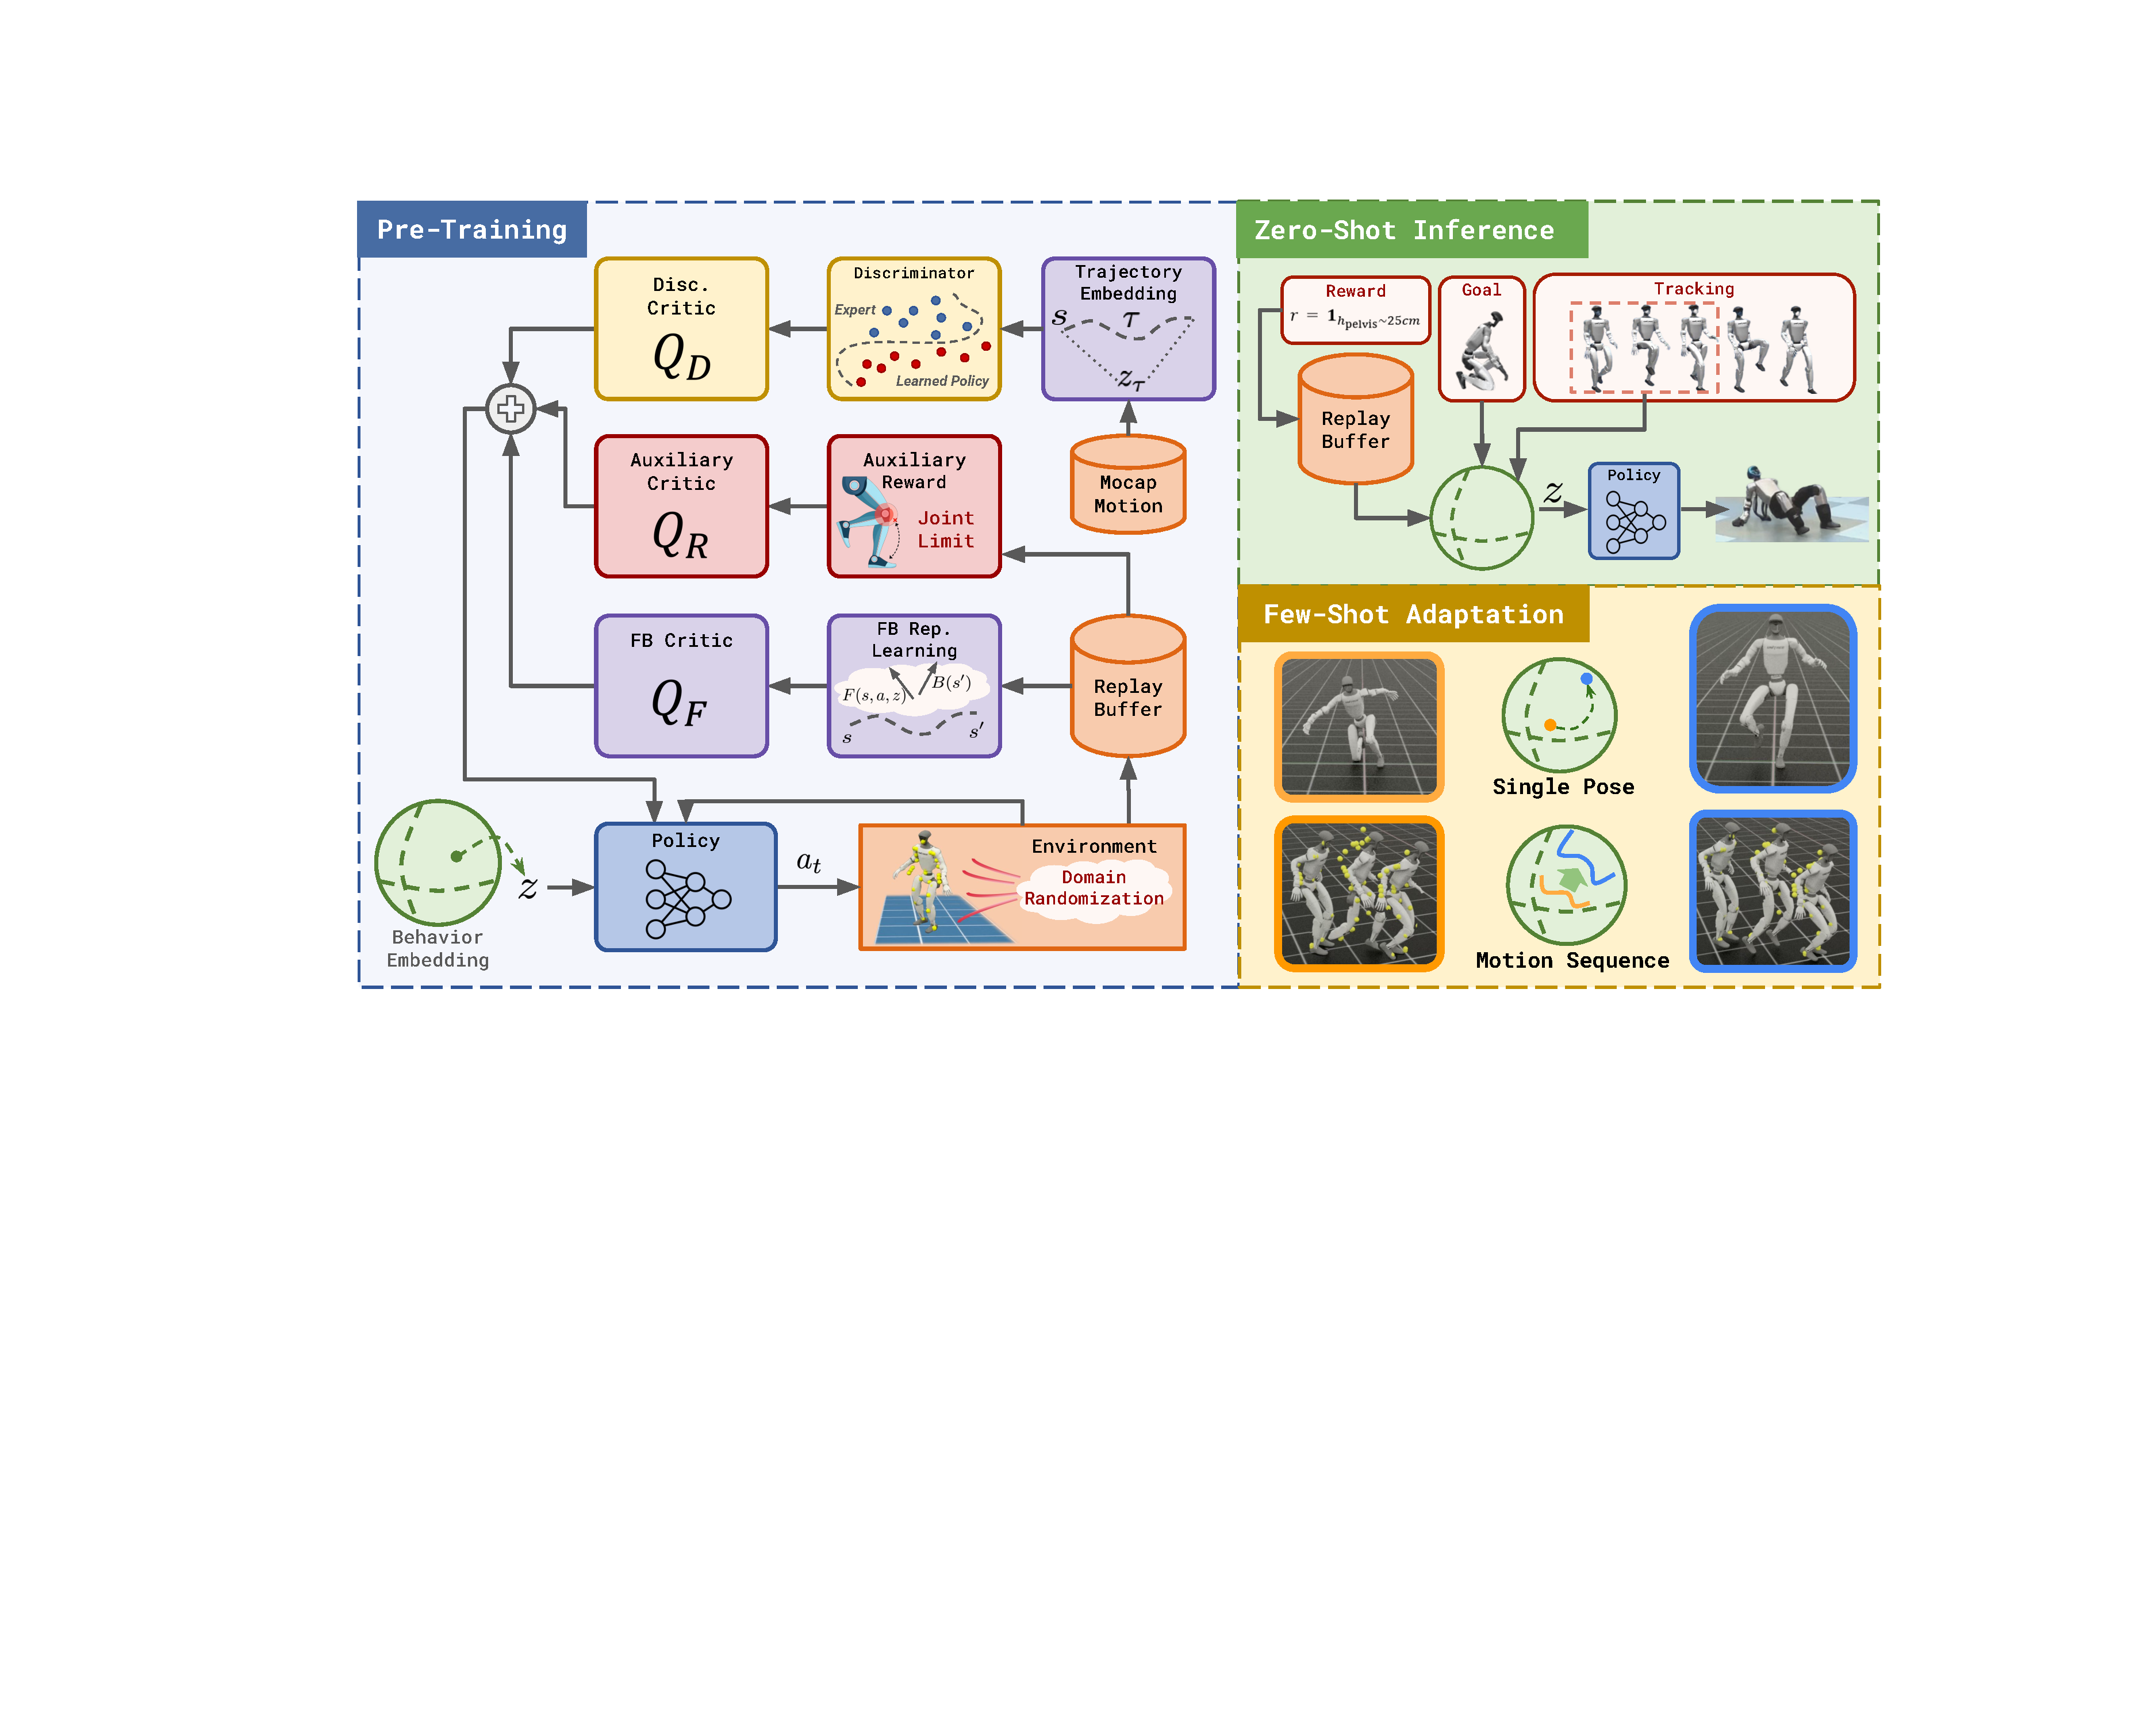
\includegraphics[width=1.0\linewidth]{image/figure_2_pipeline_2col.pdf}}
    \vspace{-0.2cm}
    \caption{\small An overview of the \method{} framework. After the pre-training stage, \method{} forms a latent space that can be used for zero-shot reward optimization, single-frame goal reaching, and tracking. It can also be adapted in a few-shot fashion to reach more challenging poses. }
    \label{fig:bfm.zero}
    \end{center}
\end{figure}

% \begin{figure}[htbp]
%     \centering
%     \includegraphics[width=0.7\textwidth]{image/figure_2_pipeline.pdf}
%     \caption{caption %\anssi{I see the symbols are clarified in the text, but I think different $s$ (proprio, priv, history) should be briefly mentioned in the caption as well.} 
%     %\guanya{I am working on this. Will do: use PDF; replace mocap data with LAFAN photos; use actual simulation image for DR.}
%     }
%     \label{fig:bfm.zero}
% \end{figure}

% \vspace{-.2in}
In this section, we outline the pipeline for training \method{} in simulation and transferring it to real humanoids. Unlike for virtual characters~\citep[e.g.,][]{peng2022ase,tessler2023calm,TirinzoniTFGKXL25zeroshot}, applying unsupervised RL to real humanoids has not yet been attempted. Our \method{} framework consists of an unsupervised pre-training stage, a zero-shot inference procedure, and possibly a fast-adaptation post-training stage (as shown in Fig.~\ref{fig:bfm.zero}). \Cref{sec:prelim} provides an overview of unsupervised RL using the forward-backward representation framework adopted by \method{}. \Cref{sec:pretrain} details \method{} pre-training, whose objective is to learn \emph{a unified latent representation} that embeds tasks (e.g., target motions, rewards, goals) into a shared space $Z \subseteq \mathbb{R}^d$ and \emph{a promptable policy} that conditions on this representation to perform diverse behaviors without task-specific retraining. Then, for downstream tasks during inference (\Cref{sec:inference}), we embed the task into the latent space and use the policy to execute the task in a zero-shot manner. We also show that we can efficiently adapt the zero-shot policy in the latent space $Z$ to improve performance on unseen tasks that are not easily covered by zero-shot inference via sampling-based optimization. % \ale{We don't really adapt the latent space itself, I would rephrase: We also show that starting from the policy obtained via zero-shot inference, we can efficiently adapt it while optimizing \textit{within} the same latent space via MPPI \cite{} and CMA-ES}


% In particular, bridging the sim-to-real gap poses significant challenges, as the dynamics differences between simulation and the real world, partial observation of the robot state, and the heterogeneous levels of hardware capabilities across humanoid platforms make direct transfer difficult. We address these challenges in the following sections and propose \method{}. 



% We address these challenges by combining domain randomization, asymmetric history-dependent training, and reward regularization into the FB-CPR algorithm. %{\color{red} On the other side, models trained for real-world deployment mostly follow a highly parallel on-policy training. We introduce changes to the training of FB-CPR to allow high-parallelization and .}

%We build on top of the recently proposed FB-CPR algorithm~\citep{TirinzoniTFGKXL25zeroshot}, which combines the FB framework reviewed in Sect.~\ref{sec:preliminaries} with a discriminator-based regularization that grounds the unsupervised RL training towards behaviors that are close to those demonstrated in a give set of motions. 
%The resulting model consists of two main components: \textbf{1)} a unified latent representation that embeds tasks (e.g., motions, rewards, goals) into a shared space, and \textbf{2)} a promptable policy that conditions on this representation to execute diverse behaviors without task-specific retraining.



% scaling factors $\beta=5$ and $\alpha_j = 0.25 \frac{\tau_{j,\max}}{k_j^p}$. $\tau_{j,\max}$ represents the maximum allowable joint torque for joint $j$

\textbf{Problem formulation.} We formulate real-world humanoid control as a partially observable Markov decision process (POMDP) defined by the tuple $(S, O, A, P, \gamma)$, where $S$ is the full state space, $O$ is the observation space, $A$ is the action space, $P(s_{t+1}|s_t,a_t)$ is the transition dynamics, and $\gamma \in (0,1)$ is the discount factor. For the 29-degree-of-freedom (DoF) humanoid, the action $a\in A \subset \mathbb{R}^{29}$ contains the proportional derivative (PD) controller targets for all DoFs. The privileged information  ($s \in \mathbb{R}^{463}$) consists of root height, body pose, body rotation, and linear and angular velocities. The observable state $o_t = \{q_t - \bar{q}, \dot{q}_t, \omega^{\mathrm{root}}_t / 4, g_t\} \in \mathbb{R}^{64}$ is defined as joint position $q_t \in \mathbb{R}^{29}$ normalized w.r.t.\ the nominal position $\bar{q}$, joint velocity $\dot{q}_t \in \mathbb{R}^{29}$, root angular velocity $\omega^{\mathrm{root}}_t \in\mathbb{R}^3$ and root projected gravity $g_t \in\mathbb{R}^3$. We denote by $o_{t,H} = \{o_{t-H}, a_{t-H},  \ldots, o_t\}\in \mathbb{R}^{93\cdot H + 64}$ the observable history composed by proprioceptive state and action. 
All the components of the states (except root height) are normalized w.r.t.\ the current facing direction and root position.
At pre-trainig, we assume that the agent has  access to a dataset of unlabeled motions $\mathcal{M} = \{ \tau\}$, which contains observation and privileged states trajectories \textit{i.e} $\tau = (o_1, s_1, \ldots, o_{l(\tau)}, s_{l(\tau)})$.  
% we use a proportional derivative (PD) controller at each joint, resulting in an action space $a \in \mathbb{R}^{29}$.

\subsection{Unsupervised RL with Forward-Backward Representations}
\label{sec:prelim}
\vspace{-2mm}
% following, we define the torque at time $t$ for joint $j$ to be
% \[
% \tau_{j,t} = k^p_j (\hat{q}_{j,t} - q_{j,t}) - k_j^d\; \dot{q}_{j,t}, \quad \hat{q}_{j,t} = \bar{q}_j + \alpha_j \beta a_{j,t}
% \]
% where $k^p_j$ and $k^d_j$ are stiffness and damping gains, $q_{j,t}$ is the robot joint state and $\dot{q}_{j,t}$ is the robot joint velocity. The joint setpoint $\hat{q}_{j,t}$ is computed based on the nominal joint configuration $\bar{q}_j$, the policy action $a_{j,t} \in [-1,1]$, and scaling factors $\beta=5$ and $\alpha_j = 0.25 \frac{\tau_{j,\max}}{k_j^p}$. $\tau_{j,\max}$ represents the maximum allowable joint torque for joint $j$.



% \textbf{Observation.} We denote by $s$ the full state (a.k.a.\ privileged information) available in simulation (but not in the real world) and by $o$ the observable state of the robot in the real world (a.k.a. proprioceptive). The privileged information  ($s \in \mathbb{R}^{463}$) consists of root height, body pose, body rotation, and linear and angular velocities. The observable state $o_t = \{q_t - \bar{q}, \dot{q}_t, \omega^{\mathrm{root}}_t / 4, g_t\} \in \mathbb{R}^{64}$ is defined as joint position $q_t \in \mathbb{R}^{29}$ $\bar{q}$, joint velocity $\dot{q}_t \in \mathbb{R}^{29}$, root angular velocity $\omega^{\mathrm{root}}_t \in\mathbb{R}^3$ and root projected gravity $g_t \in\mathbb{R}^3$. We denote by $o_{t,H} = \{s^p_{t-H}, a_{t-H},  \ldots, s^p_t\}\in \mathbb{R}^{93\cdot H + 64}$ the observable history composed by proprioceptive state and action. All the components of the states (except root height) are normalized w.r.t.\ the current facing direction and root position~\citep{WonGH22,Luo2023phc,TirinzoniTFGKXL25zeroshot}.

% builds on top of the recently proposed FB-CPR algorithm~\citep{TirinzoniTFGKXL25zeroshot},

During the pretraining phase, \method{} learns a compact representation of the environment by observing online reward-free interactions in the simulator and leveraging an offline dataset of unlabeled behaviors, resulting in a model that can be prompted to tackle a wide range of downstream tasks (e.g., tracking or reward maximization) in a zero-shot manner. To achieve this, we build on top of the recent FB-CPR algorithm~\citep{TirinzoniTFGKXL25zeroshot} which combines the Forward-Backward (FB) method for zero-shot RL \citep{Touati21fb} with online training and policy regularization on motion-capture data. This method falls in the broader category of unsupervised RL based on successor features~\citep[e.g.,][]{Touati21fb,touatizerorl,Pirotta24fastimitation,park2024foundation,agarwal2024proto}, which involves three components: (i) a latent task feature $\phi: S \rightarrow \mathbb{R}^d$ that embeds observation $s \in S$ into a $d$-dimensional vector, (ii) a policy $\pi_z: S\rightarrow A$  conditioned on a latent vector $z \in \mathbb{R}^d$, and (iii) latent-conditioned successor features~\citep{barreto2017successor} $F_z$ that encode the expected discounted sum of latent task features under the corresponding policy $\pi_z$, i.e, $F_z \simeq \mathbb{E}[\sum_{t} \gamma^t \phi(s_t)\mid \pi_z ]$. We now explain how FB-CPR trains those components.


% The representation $\phi$ defines a latent task space by inducing a family of linear reward functions of the form, i.e., $r_z(s) = \phi(s)^\top z$, which are used as \textit{unsupervised signal} to train the policy family. In particular, each policy $\pi_z$ is optimized to maximize $\mathbb{E}[ \sum_t \gamma^t r_z(s_t) \mid \pi_z]$, which can be equivalently expressed as $\mathbb{E}[ \sum_t \gamma^t \phi(s_t)^\top z \mid \pi_z] \simeq F_z^\top z$. Intuitively, $z \in Z$ defines a \emph{task-centric} latent space associated with the task feature $\phi$, where for each $z$, the corresponding $\pi_z$ optimizes the linear combination of $\phi$, $r_z=\phi^\top z$. As shown in \Cref{sec:latent}, the $Z$ space learned by \method{} is smooth, explainable, and semantically meaningful and enables both zero-shot inference and few-shot adaptation. Importantly, in contrast to standard RL approaches, $r_z$ is not given (e.g., motion tracking) but learned. Therefore, it can represent a wide range of tasks.

\textbf{FB representations and FB-CPR.} Among the different unsupervised RL approaches, forward-backward (FB) representations provide a principled unsupervised training objective for jointly learning latent task representations and their associated successor features. At a high level, FB learns a finite-rank approximation of long-term policy dynamics, where $\backward$ captures the low-frequency features that best summarize the long-range temporal dependencies between states.  Formally, given a training state distribution $\rho$, the FB framework learns two mappings: a forward mapping $\forward: S \times A \times \mathbb{R}^d \rightarrow \mathbb{R}^d$ and a backward mapping $\backward: S \rightarrow \mathbb{R}^d$ such that the long-term transition dynamics induced by the policy $\pi_z$ decompose as:
\begin{equation}~\label{eq:fb_def}
    M^{\pi_z}(\mathrm{d}s' \mid s, a) \simeq \forward(s, a, z)^\top \backward(s') \rho(\mathrm{d}s')
\end{equation}
where for any region $X \subset S$ of the state space, $M^{\pi_z}(s' \in X \mid s, a) := \sum_{t} \gamma^t \mathrm{Pr}(s_t \in X \mid s, a, \pi_z)$ denotes the discounted visitation probabilities of reaching $X$ under the policy $\pi_z$, starting from the state-action pair $(s, a)$. Eq.~\ref{eq:fb_def} implies that $\forward$ is the successor features of $\phi(s) := ( \mathbb{E}_{\rho}[\backward(s) \backward(s)^\top])^{-1} \backward(s)$~\citep{touatizerorl}.
The learned representation $\phi$ defines a latent task space by inducing a family of linear reward functions of the form, i.e., $r_z(s) = \phi(s)^\top z$, In particular, each policy $\pi_z$ is optimized to maximize $\mathbb{E}_{\rho}[\sum_t \gamma^t \phi(s_t)^\top z \mid \pi_z] = \forward(s,a,z)^\top z$, i.e., $\forward(s,a,z)^\top z$ is a Q-value function of $\pi_z$ with reward $r=\phi^\top z$. Intuitively, $z \in Z$ defines a \emph{task-centric} latent space associated with the task feature $\phi$, where for each $z$, the corresponding $\pi_z$ optimizes the linear combination of $\phi$, $r_z=\phi^\top z$. As shown in \Cref{sec:latent}, the $Z$ space learned by \method{} is smooth and semantic, and it enables both zero-shot inference and few-shot adaptation. Importantly, in contrast to standard RL approaches, the set of reward functions of interest $\{r_z\}$ is not given (e.g., motion tracking) but learned, and it can represent a wide range of tasks. 
%
FB-CPR~\citep{TirinzoniTFGKXL25zeroshot} extends the general FB framework by introducing a latent-conditioned discriminator to regularize the unsupervised learning process to produce policies that are close to a set of demonstrated behaviors in a motion dataset $\mathcal{M}$. Furthermore, while FB algorithm is offline, FB-CPR is trained fully online and off-policy and does not require a full-coverage offline dataset.
% This means that for each $z$, $\mathbb{E}_{\rho}[\sum_t \gamma^t \phi(s_t)^\top z \mid \pi_z] = \forward(s,a,z)^\top z$, i.e., $\forward(s,a,z)^\top z$ is a Q-value function of $\pi_z$ with reward $r=\phi^\top z$. 
%
% \paragraph{Zero-shot generalization to new tasks}
% Given an \emph{arbitrary} reward function $r(s)$, the corresponding Q function of $\pi_z$ can be formulated as 

% \begin{align}
%     Q_r^{\pi_z}(s,a) &= \mathbb{E}[\sum_t \gamma^t r(s_t)] = \int_{s'} M^{\pi_z}(\mathrm{d}s' \mid s, a) r(s') \\ 
%     &\simeq \int_{s'} \forward(s,a,z)^\top \backward(s') r(s') \rho(\mathrm{d}s')=
%     \forward(s,a,z)^\top \int_{s'} \backward(s') r(s') \rho(\mathrm{d}s')
% \end{align}

% Since $\forward(s,a,z)^\top z$ is the Q function of $\pi_z$, we have $z_r = \sum_{s} \backward(s) r(s)$. In other words, once the FB representations are learned, for any new tasks with reward $r$, the corresponding latent vector $z_r$ and the policy $\pi_{z_r}$ can be efficiently computed in a \emph{zero-shot} way. For example, for a goal-reaching task where $r(s)=\mathbbm{1}(s=s_g)$, we have $z_r=B(s_g)$. 

% \begin{align}
% Q_r^\pi(s,a) = E[\sum_{t}\gamma^t r_{t+1}] = \sum_{s'} M^\pi(s'|s,a) r(s') =
% \sum_{s'} F^\pi(s,a) B(s') r(s') =
% F^\pi(s,a) \sum_{s'} B(s') r(s') = 
% F^\pi(s,a) z_r
% \end{align}
%
% \paragraph{Zero-shot reward inference} Given a new reward function $r(s)$, the goal of reward inference is to find a latent vector $z \in Z$ such that 
% \begin{equation}
%     r(s) \approx \phi(s)^\top z = \backward(s)^\top (\mathbb{E}_{\rho}[\backward(s) \backward(s)^\top])^{-1} z 
% \end{equation}
%
% Example for goal reaching: When $z = B(s_i)$, the corresponding reward is 
% \begin{equation}
%     \phi(s)^\top \backward(s_i) = \backward(s)^\top (\sum_{i=1}^N \frac{1}{N} \backward(s_i) \backward(s_i)^\top)^{-1} \backward (s_i)
% \end{equation}
%
% At a high level, FB learns a finite-rank approximation of long-term policy dynamics, where $\backward$ captures the low-frequency features that best summarize the long-range temporal dependencies between states. 
% In \Cref{sec:pretrain}, we train FB within an off-policy actor-critic scheme, where the forward and backward mappings are trained using a temporal-difference loss~\citep{blier2021learning}, while the policies are updated via deterministic policy gradients.  










% ================== Current Version ==================


% At the pretraining stage, \method{} aims to learn an interpretable latent space that can be zero-shot applied to tasks like tracking and reward-maximizing, as well as being efficiently adapted to challenging cases. 
% To achieve this, we adopt a TD-based actor-critic algorithm for unsupervised RL ~\citep[e.g.,][]{Touati21fb,touatizerorl,Pirotta24fastimitation,TirinzoniTFGKXL25zeroshot,park2024foundation,agarwal2024proto,jajoo2025regularized} and learns a forward mapping $\forward$, a backward mapping $\backward$, a policy (actor) $\actor$, and three critics to optimize the latent space: a forward-backward $\fbcritic$ for learning the latent representation, a discriminator $\disccritic$ for learning human-like behavior, and an auxiliary critic $\auxcritic$ for regulating the learned policy behaviors for sim-to-real transfer. \yitang{I think we can make this part more intuitive} 


% Formally, \method{}  builds on the notion of successor features~\citep[e.g.,][]{barreto2017successor} and first learns a forward $\forward$ and backward mapping $\backward$ to approximate a low-rank decomposition of the dynamics of the learning policies. Given a class of reward functions, $R_\phi = \{r(s) = \phi(s)^\top z_r\}$, the Q-values for any reward $r(s) = \phi(s)^\top z_r$ can be written as
% \begin{equation}
%     Q^\pi_r(s,a) = \int_{s' \in S} M^\pi(\mathrm{d}s' \mid s, a) \phi(s')^\top z_r 
% % =\mathbb{E}_{s^+\sim M^\pi(\cdot|s,a)}\big[\phi(s^+)\big]^\top z_r 
% =  \forward ^\pi(s,a)^\top z_r,
% \end{equation}

% where, $\forall \mathcal{X} \subseteq S$, $M^\pi(\mathcal{X} |s,a) = \sum_{t=0}^\infty \gamma^t \mathrm{Pr}(s_t \in \mathcal{X}| s,a,\pi)$ is the successor measure, $\forward^\pi(s,a)$ is the successor features of $\pi$, i.e., the average of the features $\phi$ associated to the states traversed by the policy. $s'$ refers to a possible future state. 
% The Forward-Backward (FB) model proposed by~\citep{Touati21fb} et of parametrized policies $\{\pi_z(s)\}_{z \in Z}$ with $z \in \mathbb{R}^d$ that are trained to be optimal for all rewards $R_\phi$, i.e.,
% \begin{equation}\label{eq:policy_opt_successor_feat}
% \pi_z(s) \approx \argmax_a \forward(s,a;z)^\top z,
% \end{equation}
% where $\forward(s,a;z)^\top z \approx Q^\star_r(s,a) = \max_{\pi}Q^\pi_r(s,a)$ and $r(s) = \phi(s)^\top z$, where the reward features $\phi$ are learned jointly with $\forward$ and the policies $\pi_z$. Combining the forward $\forward$ and $\backward$ mapping, we approximate the dynamics of the policy: 
% \begin{equation}\label{eq:fb_approx}
% F(s,a;z)^\top B(s') \approx M^{\pi_z}(ds'|s,a)
% \end{equation}
% that when combined with Eq.~\ref{eq:policy_opt_successor_feat} leads to $\phi(s) = \mathbb{E}_s[\backward(s)\backward(s)^\top]^{-1} \backward(s)$. 
% Intuitively, the FB algorithm implements an \textit{inductive bias} to jointly train policies and rewards, where the policies are optimal for the rewards, and the rewards can be expressed as linear functions of features $B$ that capture the ``low-frequency'' dynamics of the policies.  In practice, an FB model is fully \emph{unsupervised} since solving Eq.~\ref{eq:fb_approx} and Eq.~\ref{eq:policy_opt_successor_feat} does not require any reward signal during training. 
% The Forward-Backward representations with Conditional Policy Regularization~\citep[FB-CPR]{TirinzoniTFGKXL25zeroshot} extends the general FB framework by introducing a latent-conditioned discriminator to regularize the unsupervised learning process to produce policies that are close to a set of demonstrated behaviors in a motion dataset.

% To optimize the forward $\forward$ and $\backward$ mappings, we learn an FB critic $\fbcritic$, which is similar to the standard Q-function in successor feature learning as $\forward(s,a;z)^\top z \approx Q^\star_r(s,a) = \argmax_{\pi}Q^\pi_r(s,a)$.  We also learn an auxiliary critic $\auxcritic$  that imposes safety and physical feasibility constraints by incorporating penalty rewards (e.g., joint limits, slippage, self-collisions). This ensures that the learned behaviors remain transferable to real humanoid hardware. Finally, we employ the discriminator critic $\disccritic$ that grounds the unsupervised training toward human-like behaviors by assigning rewards based on a latent-conditioned discriminator. This prevents the policy from drifting to unrealistic motions and aligns it with the distribution of demonstrated trajectories. At the pre-training stage, we use a dataset of unlabeled motions $\mathcal{M} = \{\tau\}$, where each motion $\tau$ is a trajectory of observations $\tau = (x_1, x_2, \ldots, x_T)$ from the retargeted LAFAN1 dataset~\citep{HarveyYNP20lafan1}. 

\subsection{BFM-Zero Pre-training for Humanoid Control}
\label{sec:pretrain}
\vspace{-3mm}
Before proceeding with the description of implementation details, we identify several design choices that are crucial for achieving sim-to-real transfer in unsupervised RL.


\textit{A) Asymmetric Training.} To bridge the gap between simulation (full state) and real robot (partial observability), we train the policy on observation history $o_{t,H}$, while critics have access to privileged information $(o_{t,H}, s_t)$. This setup improves policy robustness under limited sensing while leveraging privileged critics to provide accurate value estimates. Using history narrows the information gap between proprioceptive actors and privileged critics and improves adaptability under domain randomization.


\textit{B) Scaling up to Massively Parallel Environments.} Inspired by recent work on large-batch off-policy RL~\citep{Seo2025fasttd3}, we scale training across thousands of environments with large replay buffers and high update-to-data (UTD) ratios. This enables efficient unsupervised training of a diverse family of policies while retaining stability, a crucial step for scaling humanoid pretraining.


\textit{C) Domain Randomization (DR).} To enhance robustness and adaptability, we randomize key physical parameters (link masses, friction coefficients, joint offsets, torso center-of-mass) and apply perturbations and sensor noise. This prevents overfitting to simulation dynamics and ensures that policies remain stable when deployed on real hardware (see  Fig.~\ref{fig:dr_and_reg} in Appendix).

\textit{D) Reward Regularization.} In robotics~\citep[e.g.,][]{he2025asap,Zakka2025mujocoplayground}, it is common to incorporate reward regularization techniques to avoid undesirable behaviors. For example, reaching the limit of the joint may lead to highly nonlinear behaviors that are difficult to model in simulation or even damage the robot's hardware.
%Please refer to Figure~\ref{fig:dr_and_reg} for a list of the penalty rewards used in our implementation and their weights.

%
% With these in mind, we can now detail the components of \method{}. \textbf{1)} A latent task space $Z \subseteq \mathbb{R}^d$ (here the unit hypersphere of radius $\sqrt{d}$); \textbf{2)} a \textit{privileged} backward embedding $\boldsymbol{B}: O \times S \to Z$ mapping states to latent task; \textbf{3)} a policy-conditional, \emph{history-based}, \emph{privileged} forward embedding $\boldsymbol{F}: (O \times A)^H \times S \times A \times Z \to \mathbb{R}^d$ that provides an estimate of the successor features under the learned policies  \textbf{4)} a promptable \emph{history-based} conditional policy $\pi: (O \times A)^H \times  Z \to A$; \textbf{5)} a \textit{privileged} latent-conditional discriminator $\boldsymbol{D}: O \times S \times Z \to \mathbb{R}$ that provides a training signal to steer the learned behaviors toward capturing behaviors represented in the motion dataset and finally the associated \emph{history-based}, \emph{privileged} critic $\disccritic: (O \times A)^H \times S \times A \times Z \rightarrow \mathbb{R}$ trained for each policy on top of the discriminator reward. We train \method{} within an off-policy actor-critic scheme, where the forward and backward mappings are trained using a temporal-difference loss~\citep{blier2021learning}, while the policies are updated via deterministic policy gradients.  


% \textit{D) Reward Regularization.} In robotics~\citep[e.g.][]{he2025asap,Zakka2025mujocoplayground}, it is common to incorporate reward regularization techniques to avoid undesirable behaviors. For example, reaching the limit of the joint may lead to highly unlinear behaviors that are difficult to model in simulation or even  to damage the robot's hardware. To address these hard constraints, we introduce an \emph{auxiliary critic} $\auxcritic(o_{t,H}, s_t, a_t,z)$ trained using a combination of penalty rewards (e.g., joint limits, feet slip, action rate, etc.) to ensure that the learned behaviors adhere to safety and operational constraints of the physical robot. This is used as an additional regularization in the policy training loss, leading to
% \[
% \ell(\pi) = - \mathbb{E}_{x \sim \mathcal{D}_{\mathrm{online}}, z\sim \nu, a \sim \pi_z(\cdot| s)} \big[ \fbcritic(x,z) + \alpha_D \disccritic(x,z)  + \alpha_R \auxcritic(x,z) \big],
% \]
% where $x=(o_{t,H}, s_t, a_t)$. Please refer to Figure~\ref{fig:dr_and_reg} for a list of the penalty rewards used in our implementation and their weights.

We train \method{} within an off-policy actor-critic scheme.
The policy-conditional, \emph{history-based}, \emph{privileged} forward map $\forward$ and \textit{privileged} backward map $\backward$ are trained to minimize the
temporal difference loss derived from the  Bellman equation for successor measures~\citep{Touati21fb}. Let $\mathcal{D}$ the replay buffer of online interactions with the simulator and $\nu$ is an arbitrary distribution over $Z$, we consider the following FB objective:
% \begin{align}\label{eq:fb.loss}
%     \mathcal{L}(F,B) &= \mathbb{E}_{\substack{z\sim\nu, (x,a,x') \sim \mathcal{D},\\ x^{+}\sim\mathcal{D}, a'\sim\pi_{z}(x')}} \Big[ \big( F(x,a,z)^\top B(x^+) - \gamma \overline{F}(x',a', z)^\top \overline{B}(x^+)\big)^2 \Big] \\
%     &\quad - 2 \mathbb{E}_{z\sim\nu, (x,a,y)\sim \rho}\big[ F(x,a,z)^\top B(y)\big],\nonumber
% \end{align}
% where $\nu$ is an arbitrary distribution over $Z$.
\begin{align*}\label{eq:fb.loss}
    \mathcal{L}(\boldsymbol{F},\boldsymbol{B}) &= \mathbb{E} \Big[ \big( \boldsymbol{F}(o_{t, H},s_t, a_t, z)^\top \boldsymbol{B}(o^{+}, s^{+}) - \gamma \overline{\boldsymbol{F}}(o_{t+1, H},s_{t+1}, a_{t+1}, z)^\top \overline{\boldsymbol{B}}(o^{+}, s^{+})\big)^2 \Big] \\
    &\quad - 2 \mathbb{E}\big[ \boldsymbol{F}(o_{t, H},s_t, a_t, z)^\top \boldsymbol{B}(o_{t+1}, s_{t+1}) \big],\nonumber
    % & \text{where } z\sim \nu, (o_{t, H},s_t, a_t, o_{t+1, H},s_{t+1}, s_{t+1}, a_{t+1}) \sim \mathcal{D}_{\mathrm{online}} \text{ and } (o^{+}, s^{+}) \sim \mathcal{D}_{\mathrm{online}} \nonumber
\end{align*}
where $z\sim \nu, (o_{t, H},s_t, a_t, o_{t+1, H},s_{t+1}) \sim \mathcal{D}$, $a_{t+1} = \pi(o_{t+1, H}, z)$ and $(o^{+}, s^{+}) \sim \mathcal{D}$. $\overline{\boldsymbol{F}}$ and $\overline{\boldsymbol{B}}$ denote the stop-gradient operator.


%
% we learn an FB critic $\fbcritic$, which is similar to the standard Q-function in successor feature learning as $\forward(s,a;z)^\top z \approx Q^\star_r(s,a) = \argmax_{\pi}Q^\pi_r(s,a)$.  The backward mapping $\boldsymbol{B}$ acts as a task encoder as well as a policy encoder. The forward map $\boldsymbol{F}$
% We also learn an auxiliary critic $\auxcritic$  that imposes safety and physical feasibility constraints by incorporating $N_{\mathrm{aux}}$ penalty rewards (e.g., joint limits, slippage, self-collisions). This ensures that the learned behaviors remain transferable to real humanoid hardware. 
The auxiliary \emph{history-based}, \emph{privileged} critic $\auxcritic$ that imposes safety and physical feasibility constraints by incorporating $N_{\mathrm{aux}}$ penalty rewards is learned with a standard Bellman residual loss:
\begin{small}
\[
\mathcal{L}(\boldsymbol{Q_R})= \mathbb{E}_{\substack{(o_{t, H}, s_t, a_t, s_{t+1}) \sim \mathcal{D}\\ z\sim\nu, a_{t+1}=\pi(o_{t+1, H}, z)}} \left[ \Big(\boldsymbol{Q_R}(o_{t, H}, s_t, a_t, z) - \sum_{k=1}^{N_{\mathrm{aux}}} r_k(s_t) - \gamma \overline{\boldsymbol{Q_R}}(o_{t+1, H},s_{t+1}, a_{t+1}, z)\Big)^2\right].
\]
\end{small}
Finally, we employ the \emph{history-based}, \emph{privileged} discriminator critic $\disccritic$ that grounds the unsupervised training toward human-like behaviors by assigning rewards based on a latent-conditioned discriminator. This acts both as a style regularization as well as a bias in the online exploration process. 
%This prevents the policy from drifting to unrealistic motions and aligns it with the distribution of demonstrated trajectories.
As in~\citep{TirinzoniTFGKXL25zeroshot}, we employ a variational representation of the Jensen-Shannon divergence and train the discriminator $\boldsymbol{D}$ with a GAN-style objective:
\begin{align*}\label{eq:disc-loss}
    \mathcal{L}(\boldsymbol{D}) = 
    -\mathbb{E}_{\substack{\tau \sim \mathcal{M}, (o, s) \sim \tau }} \left[ \log(\boldsymbol{D}(o, s, z_\tau))\right] -\mathbb{E}_{\substack{(o, s, z) \sim \mathcal{\boldsymbol{D}}}} \left[\log(1 - \boldsymbol{D}(o, s, z))\right].
\end{align*}
where $z_\tau=\frac{1}{l(\tau)} \sum_{(o,s) \in \tau} \boldsymbol{B}(o,s)$ is a zero-shot imitation embedding of the motion $\tau$. We can then fit a \emph{style} critic $\disccritic$ with a Bellman residual loss similar to the auxiliary critic with a reward $r_d(o_t,s_t,z)=\frac{\boldsymbol{D}(o_t,s_t,z)}{1-\boldsymbol{D}(o_t,s_t,z)}$.
% \[
% \mathcal{L}(\boldsymbol{Q_D}) = \mathbb{E} \left[ \Big(\boldsymbol{Q_D}(o_{t, H}, s_t, a_t, z) - \frac{\boldsymbol{D}(o_t,s_t,z)}{1-\boldsymbol{D}(o_t,s_t,z)}  - \gamma \overline{\boldsymbol{Q_D}}(o_{t+1, H}, s_{t+1}, a_{t+1}, z)\Big)^2\right]
% \]
Bringing together these critiques results in the final actor loss. % for \method{},
\begin{equation*}\label{eq:actor_loss}
    \mathcal{L}(\pi) = - \mathbb{E}_{\substack{(o_{t, H},s_t) \sim \mathcal{D}\\
    a_{t} = \pi(o_{t, H}, z), z \sim \nu, }} \Big[ \boldsymbol{F}(o_{t, H}, s_t,a_t, z)^\top z + \lambda_D \boldsymbol{Q_D}(o_{t, H}, s_t,a_t, z) + \lambda_R \boldsymbol{Q_R}(o_{t, H}, s_t,a_t, z)\Big].
\end{equation*}
% At the pre-training stage, we use a dataset of unlabeled motions $\mathcal{M} = \{\tau\}$, where each motion $\tau$ is a trajectory of observations $\tau = (x_1, x_2, \ldots, x_T)$ from the retargeted LAFAN1 dataset~\citep{HarveyYNP20lafan1}. T
% The overall structure of \method{} pre-training is summarized in Fig.~\ref{fig:bfm.zero}. %We refer the reader to Appendix~\ref{} for details about the training procedure.



%
% \ale{Add details of what is in $s^p$ and what is in $s^v$?} More precisely, the model inputs are as follows:
% \begin{itemize}
%     \item The critics $F$, $Q_D$, and $Q_R$ take as input the full state $(s^p_t, s^o_t)$ and the last action $a_{t-1}$ over a $H$-step window. Let $x_t = (s^p_t, s^o_t, a_{t-1})$ be the extended state, then input of the critics is $s_{\mathrm{critic},t} = (x_t, x_{t-1}, \ldots, x_{t-H+1})$.
%     \item The backward map $B$ and the discriminator $D$ receives in input the full state, i.e., $s_t = (s^p_t, s^o_t)$. We don't use actions since they are not available in the unlabeled dataset of behaviors. We don't use history for these models.
%     \item The policy $\pi$ is provided with the proprioceptive state and the last action, i.e., $y_t = (s^p_t, a_{t-1})$, but no privileged state. Similarly to the critic we use a $H$-step window leading to $s_{\mathrm{policy},t} = (y_t, y_{t-1}, \ldots, y_{t-H+1})$
% \end{itemize}
%


% \begin{table}[t]
% \begin{wraptable}{l}{.4\textwidth}
%     \resizebox{.4\textwidth}{!}{%
%     \begin{tabular}{|c|c|}
%         \hline 
%         % Parameter & Range \\
%         % \hline\hline
%         \multicolumn{2}{|c|}{Dynamics Randomization} \\
%         \hline
%         COM \emph{displacement} [m] & $\mathcal{U}([-0.02, 0.02])$\\
%         Link mass \emph{multiplier} & $\mathcal{U}([0.95, 1.05])$\\
%         Friction & $\mathcal{U}([-0.5, 1.25])$\\
%         \makecell{Nominal joint position\\ \emph{displacement} [m]} & $\mathcal{U}([-0.02, 0.02])$\\
%         External perturbation [m/s] & $\mathcal{U}([0, 0.5])$\\
%         \hline
%         \hline
%         \multicolumn{2}{|c|}{Additive Observation Noise} \\
%         % \hline
%         % Parameter & Range\\
%         \hline
%         $q_t - \bar{q}$ & $\mathcal{U}([-0.01, 0.01])$\\
%         $\dot{q}_t$ & $\mathcal{U}([-0.5,0.5])$\\
%         $\mathrm{grav}_t$ & $\mathcal{U}([-0.05,0.05])$\\
%         $\dot{\omega}^{\mathrm{root}}_t / 4$ &  $\mathcal{U}([-0.05,0.05])$ \\
%         \hline
%     \end{tabular}
%     }
%     \caption{Dynamics randomization and observation noise.}
%     \label{tab:dr}
% % \end{table}
% \end{wraptable}






% \paragraph{Environment parallelization.} 
% The majority of humanoid approaches trained for real-world deployment leverages highly-parallel on-policy training on hundreds million of environment interactions. While this approach is effective to train a single policy, we argue that off-policy learning is preferable when training a full set of parameterized policies. We take inspiration from the recipe in FastTD3~\citep{Seo2025fasttd3} to scale up unsupervised off-policy RL to using massively parallel environments. Similarly to FastTD3, we use standard MLPs for all the components of the model, even for handling history. The policy size is just XXX M parameters. We scale the buffer size accordingly to the number of environments, following the rule $N \times N_{env} \times H_{episode}$. We use a batch size of $1024$ and we use an update-to-data ratio of $N_{\mathrm{grad}}=16$ gradient steps per (parallel) environment step.
% %
% As we increase the number of training environments, we adapt the strategy for online interaction in simulation. The original FB-CPR deploys collects data by unrolling random policies (i.e., sampling $z$ uniformly from $Z$) that are switched every $N_{\mathrm{rnd}}$ steps. We augment this strategy by deploying policies inferred through tracking inference in $p_{\mathrm{track}}$\% of the environments and switch them every $N_{\mathrm{track}}$ steps. Concretely we samples slices of $N_{\mathrm{track}}$ steps from the motion dataset $\mathcal{M}$ and infer a sequence of policies $\{z_1, z_2, \ldots, z_{N_{\mathrm{track}}}\}$ to track them. These policies are then used to control the robot for $N_{\mathrm{track}}$ steps from the current state of the simulator. This simple change allows to collect more informative data both for the discriminator and for the auxiliary reward. For example, using highly-frequently switching policies we are able to better control rewards such as action rate or joint limits. \matteo{We could also deploy goal reaching policies in some environments. We should try this.} \matteo{Keep or remove it based on what we really deploy and use for the experiments.}




































% {\color{blue}
% [META very rough attempt]


% In this section we detail the pipeline for training a behavioral foundation model in simulation and transferring it zero-shot to a real robot. We build on top of the recently proposed FB-CPR algorithm~\citep{TirinzoniTFGKXL25zeroshot}. This approach consists of two main components: (1) a unified latent representation that embeds tasks (eg., motions, rewards, goals) into a shared space, and (2) a promptable policy that conditions on this representation to execute diverse behaviors without task-specific retraining.

% While this approach has been successfully used to train a model for virtual character animation in simulation, bridging the virtual-robot gap presents a significant challenge. First, models pre-trained in simulation step should be adapted to facilitate the transfer of the policy to the real robot (sim2real gap). Second, the distinction between full-observability in simulated environments and the limited, often partial, observability encountered in real-world scenarios necessitates the development of novel training methodologies (observation gap). Third, real robots come with several hardware constraints and requirements to preserve the robot's longevity and minimize wear, tear, or even damage. For instance, it is crucial to avoid high-frequency oscillations in the control signals to prevent motor overheating.
% We address these challenges through a combination of domain randomization, asymmetric training and reward regularization.

% \paragraph{Domain randomization.} Domain randomization is used in RL to enhance an agent's robustness by training it across a distribution of similar environments. This approach has proven crucial for addressing
% the sim-to-real gap in RL~\citep[e.g.,][]{PengAZA18,ChebotarHMMIRF19,Kaidanov2024theroleofdr,he2025asap}, enabling zero-shot transfer of policies from simulation to the real world.
% We apply domain randomization to various \emph{physical parameters} of the simulated robot, including mass, friction coefficients, default joint positions  $\bar{q}$ (for both actions and observations, effectively simulating joint offset
% calibration errors), and the torso's center of mass position. We also apply \emph{perturbation randomization} by applying force perturbations of random amplitude to the robot's torso. The primary objective of perturbation randomization is to destabilize the robot's state, compelling it to adapt and learn effective recovery strategies from unstable conditions. Additionally, we introduce \emph{noise to the robot's proprioceptive information} to mimic real-world sensor inaccuracies. This comprehensive randomization strategy ensures that the policy learns to operate effectively under a wide range of conditions, thereby improving its robustness when deployed on the physical robot.


% \paragraph{Asymmetric training.} Asymmetric training~\citep[e.g.,][]{Kaidanov2024theroleofdr,he2025asap} is a technique used to bridge the gap between the full observability available in simulation and the limited, often partial, observability encountered in real-world scenarios. In this approach, the policy is trained using only the information that will be available during deployment, while the critics have access to additional privileged information. This setup allows the critics to provide more accurate estimates, which can help guide the policy's learning process. Informally, we implement asymmetric training by providing the policy with only proprioceptive information $s^p_t$, while the critics have access to both proprioceptive and privileged information $s_t = (s^p_t, s^v_t)$. This approach helps the policy learn to operate effectively with limited information, improving its performance when transferred to the real robot.


% \paragraph{Reward Regularization.} It is common in robotics~\citep[e.g.][]{he2025asap,Zakka2025mujocoplayground} to incorporate reward regularization techniques to encourage desired behaviors and discourage undesirable ones. For example, reaching the limit of the joint may lead to highly unlinear behaviors that are difficult to model in simulation or worse damage the robot's hardware. To address these hard constraints, we modify the FB-CPR framework by introducing an auxiliary critic trained using a combination of penalty rewards (e.g., joint limits, feet slip, action rate, etc.).




% \subsection{Zero-shot Inference and Few-Shot Adaptation}
% \label{sec:inference-and-adaption}

\textbf{Zero-shot inference.} \label{sec:inference}At test time, \method{} can be used to solve different tasks in \emph{zero-shot} fashion, i.e., without performing additional task-specific learning, planning, or fine-tuning. Given an \emph{arbitrary} reward function $r(s)$, the corresponding Q function of $\pi_z$ can be formulated as 
%
\begin{small}
\begin{align*}
    Q_r^{\pi_z}(s,a) &= %\mathbb{E}[\sum_t \gamma^t r(s_t)] = 
    \int_{s'} M^{\pi_z}(\mathrm{d}s' | s, a) r(s')
    \simeq \mathbb{E}_{s'\sim \rho} [ \forward(s,a,z)^\top \backward(s') r(s')] =
    \forward(s,a,z)^\top \mathbb{E}_{s'\sim \rho} [ \backward(s') r(s')].
\end{align*}
\end{small}
%
Since $\forward(s,a,z)^\top z$ is the Q function of $\pi_z$, we have $z_r = \mathbb{E}_{s'\sim \rho}[\backward(s) r(s)]$. 
In practice, we can leverage a sample-based estimate, given by $z_r =\frac{1}{N} \sum_i r(s_i) \backward(s_i)$ where $s_i \in \mathcal{D}$ and $\mathcal{D} = \{(s_i,r_i)\}$ is obtained by subsampling the online replay buffer. 
For a goal-reaching task, we have $z_g=B(s_g)$. 
Finally, for \textbf{tracking} a motion $\tau=\{s_1,\ldots,s_n\}$, a sequence of policies $\{z_t\}$ is obtained as $z_t = \sum_{t'=t}^{t+H} \backward(s_{t'})$, where $H$ is a look-ahead horizon~\citep{Pirotta24fastimitation}. 

\textbf{Few-Shot Adaptation.}
\label{sec:adaption}We can leverage optimization techniques for adaptation in latent space $Z$ using online interaction with the simulator at test time.
% To address zero-shot is suboptimal due to some environment variance, we 
We demonstrate this by refining a static pose or an entire motion to maximize $J(z)=\sum_{t=0}^{T-1}\Big(r_{\text{task}}(s_t)-\alpha_{R}\textstyle\sum_{k=1}^{N_{\text{aux}}}r_k(o_t,s_t,a_t)\Big)$. For \textbf{single-pose adaptation}, we use the zero-shot policy $z_0 = B(s_g, o_g)$ as initial point and apply the Cross-Entropy Method (CEM)~\citep{rubinstein1999cross,rubinstein2004cross}. 
% \matteo{Because the policy is history-conditioned and promptable, $\pi(o_{t,H},z)$, the resulting $z^\star$ captures the altered inertial response without retuning the network parameters, and retains the human-like prior induced by the discriminator pathway used during training.}
For \textbf{trajectory-level adaptation}, we warm-start from a tracked motion sequence and perform zero-order, sampling-based trajectory optimization over a \emph{sequence} of latent prompts, $\mathbf z_{t:t+H-1}$, using a dual-loop annealing schedule in the spirit of DIAL-MPC \citep{xue2025full}. This procedure consistently stabilizes challenging segments and reduces motion-tracking error, while retaining the human-like prior given by the discriminator without finetuning networks.




% \section{Few-Shot Adaptation atop BFM-Zero}
% \subsection{Efficient Searching-based optimization}
% \subsection{Efficient High Level Planning}